\documentclass[11pt]{article}

\usepackage{subfigure,fancybox,epsfig,enumerate,amssymb,amsmath,amsthm,
fullpage,pst-plot,pstricks, arcs,tikz,hyperref,pstricks-add, graphicx}
\graphicspath{{images/}}


\newcommand{\A}{\ensuremath{\mathcal A}}
\newcommand{\B}{\ensuremath{\mathcal B}}
\newcommand{\F}{\ensuremath{\mathcal F}}
\newcommand{\C}{\ensuremath{\mathbb C}}
\newcommand{\K}{\ensuremath{\mathbb K}}
\newcommand{\R}{\ensuremath{\mathbb R}}
\newcommand{\Z}{\ensuremath{\mathbb Z}}
\newcommand{\defn}[1]{\textbf{#1}}
\newcommand{\ray}[1]{\overrightarrow{#1}}
\renewcommand{\line}[1]{\overleftrightarrow{#1}}
\newcommand{\segment}[1]{\overline{#1}}

\newtheorem{theorem}{Theorem}[section]
\newtheorem{lemma}[theorem]{Lemma}
\newtheorem{corollary}[theorem]{Corollary}
\newtheorem{claim}[theorem]{Claim}
\newtheorem{conjecture}[theorem]{Conjecture}
\newtheorem{prop}[theorem]{Proposition}


\theoremstyle{definition}
\newtheorem{definition}[]{Definition}
\newtheorem{observation}[theorem]{Observation}
\newtheorem{example}[theorem]{Example}
\newtheorem{note}[theorem]{Note}
\newtheorem{notation}[theorem]{Notation}
\newtheorem{ack}{Acknowledgements}
\newtheorem{axiom}{Axiom}
\newtheorem{problem}[theorem]{Problem}
\newtheorem{question}[theorem]{Question}
\newtheorem{aaxiom}{Axiom A}



\begin{document}
%This is where the fun begins!


\title{Josh \& Danny}

\maketitle

\section{Glide Reflections}
Now we will introduce the concept of a Glide Reflection, and prove which
combinations of isometries are equivalent to a single Glide Reflection.

As we saw in a precious section, three Reflections can create any isometry of
the plane where the orientation is reversed. In the case where all three lines
are parallel, they can be reduced to a single reflection, but in the case where
there are at least two points of intersection among the lines of Reflection,
they represent an operation that cannot be reduced into a single one of any of
the isometries that we have introduced; therefore we will reduce them to a
representation where each operation has a unique identity and refer to this
class of isometries as Glide Reflections.

\begin{theorem}\label{Glide Reflection}
  A Glide Reflection is a form of isometry represented by a composition of a
reflection and a translation parallel to the line of reflection; it is a
fundamental isometry which cannot be further reduced into any single component.
\end{theorem}

The irreducibility of a Glide Reflection will be easy to see, but first we will
look at how a Glide Reflection can be formed from three reflections, as this
will demonstrate the reasons for our choice of representation.

\begin{theorem}\label{3 Reflections form a Glide Reflection}
  A Glide Reflection can be formed from three Reflections, as long as the
  lines of reflection have at least two points of intersection among them.
\end{theorem}

First we will consider the case where two of the reflection lines are parallel,
but first we need a supporting theorem which will be required to completely
reduce the Reflections:

\begin{theorem}\label{Glide Reflection from a Reflection and a Translation}
  A Glide Reflection can be formed from one Reflection and one Translation,
  as long as the angle between the reflection line and translation vector is
  not 90 degrees.
\end{theorem}

\begin{proof}
  A Reflection and a Translation perpendicular to each other can be combined by
  moving the Reflection by half of the Translation's magnitude in the opposite
  direction.



  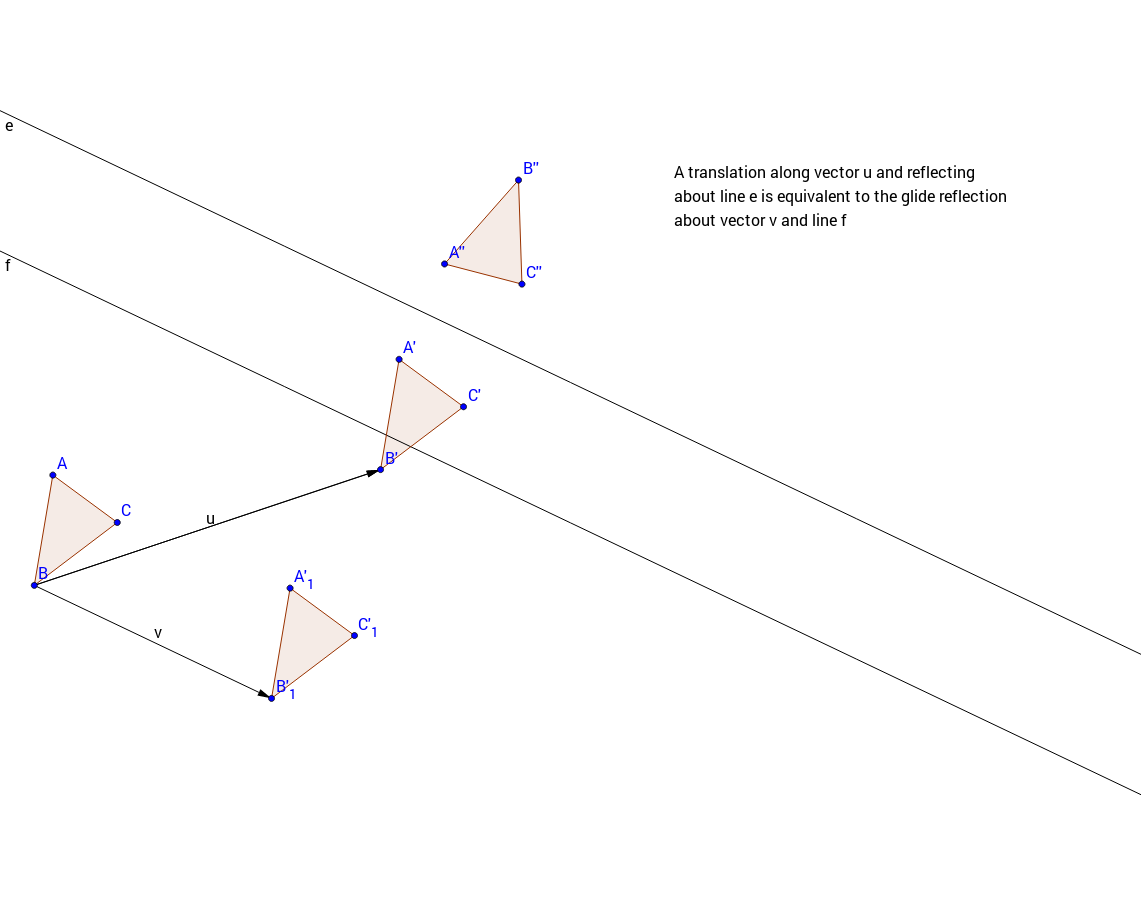
\includegraphics[scale=.4]{glide}



  Therefore, a reflection line and a translation vector with an arbitrary angle
  between them can be reduced to a Glide Reflection by taking the components of
  the translation vector both parallel and perpendicular to the reflection
  line; the perpendicular component can be absorbed by moving the reflection
  line, and since the parallel component must be non-zero due to the
  restriction on the angle of the translation vector, the remaining two
  isometries make up our definition of a Glide Reflection.
\end{proof}

Now we can prove Theorem 5.2 for the following case:

\begin{proof}
  For a set of Reflection lines $L_{1}$, $L_{2}$, and $L_{3}$, where the first
  two are parallel and the third intersects both, they can be reduced to a
  Glide Reflection by combining the parallel reflection lines into a single
  Translation. The resulting translation vector will never be at a 90 degree
  angle with the remaining reflection line because that reflection line started
  off at some angle with respect to the other two reflection lines, and as
  shown above, this forms a Glide Reflection.
\end{proof}

In order to show that any three Reflections can be made into a Glide
Reflection even if none are parallel, we leverage the fact that two
intersecting Reflections form a Rotation.

\begin{proof}
  For a set of Reflections across lines $L_{1}$, $L_{2}$, and $L_{3}$, where
  there are at least two intersection points, the isometries can be reduced to
  a Glide Reflection by coercing two of the reflection lines such that one of
  them is parallel to the third. This can be done because two intersecting
  reflection lines compose to form a Rotation around the intersection point:
  First transform the two Reflections into the Rotation, then choose a new
  Reflection line through the center of Rotation that is parallel to the third
  Reflection line. It is guaranteed that a Reflection line exists such that
  when composed with the Reflection line that you chose it will reproduce the
  Rotation around that center point. Now that the lines that formed the
  Rotation have been transformed, you have reached the case where two
  Reflection lines are parallel and the third intersects both, which we have
  already shown to be a Glide Reflection.
\end{proof}

\subsection{Exercises}

Now that we've introduced the concept of Glide Reflections, there are a few
things which can increase your understanding of them and other isometries:
\begin{enumeration}
\item Add a column for "Glide Reflections" to your composition table. Are there
  compositions you couldn't do before that are simpler with Glide Reflections?
  What sorts of compositions can you have with Glide Reflections?
\item Prove that the reflection and translation used to make a Glide Reflection
  commute with each other, so there is no need for ordering them.
\item Why do we require the translation to be parallel to the reflection line?
  What properties do we gain by doing so? What would it mean for Glide
  Reflections if we didn't require this?
\end{enumeration}

\end{document}
